\chapter{Implementación \newline (Primer iteración)}\label{ch:Implementación}
El propósito de la elaboración del primer prototipo fue construir pequeños módulos funcionales para hacer pruebas unitarias con ellos y, posteriormente, integrados para garantizar su interoperatividad. Debido a la complejidad técnica del proyecto y la necesidad de utilizar diversas bibliotecas, surgieron dudas sobre si estas herramientas funcionarían de manera correcta e integrada. Además, al ser un proyecto desarrollado por un único miembro, cualquier problema podría comprometer el avance y la viabilidad del proyecto. Este enfoque permitió validar el funcionamiento independiente de cada módulo y asegurar que el proyecto pudiera avanzar sin bloqueos técnicos.
El desarrollo del primer prototipo siguió una serie de etapas que se describen a continuación:

\section{Construcción inicial del Canvas con JavaScript}
EL primer punto clave que se atacó del proyecto fue la implementación de todo el plano donde se hará la visualización interactiva de las funciones y series, para esto, se se usó el elemento \texttt{<canva>} de HTML, y fué modificado meramente con Javascript para darle su funcionalidad.

\subsection{Funciones para graficar funciones y series de Fourier}
Para lograrlo, se modifico el componente \texttt{<canva>} desde Javascript (véase \hyperref[app3:canva_js]{Apéndice C}) para lograr dibujar el lienzo y darle toda su funcionalidad de poder moverse y hacer zoom en él. Además de funciones para poder dibujar sobre ese lienzo gráficas de funciones y series de funciones.
\begin{figure}[H]
	\centering
	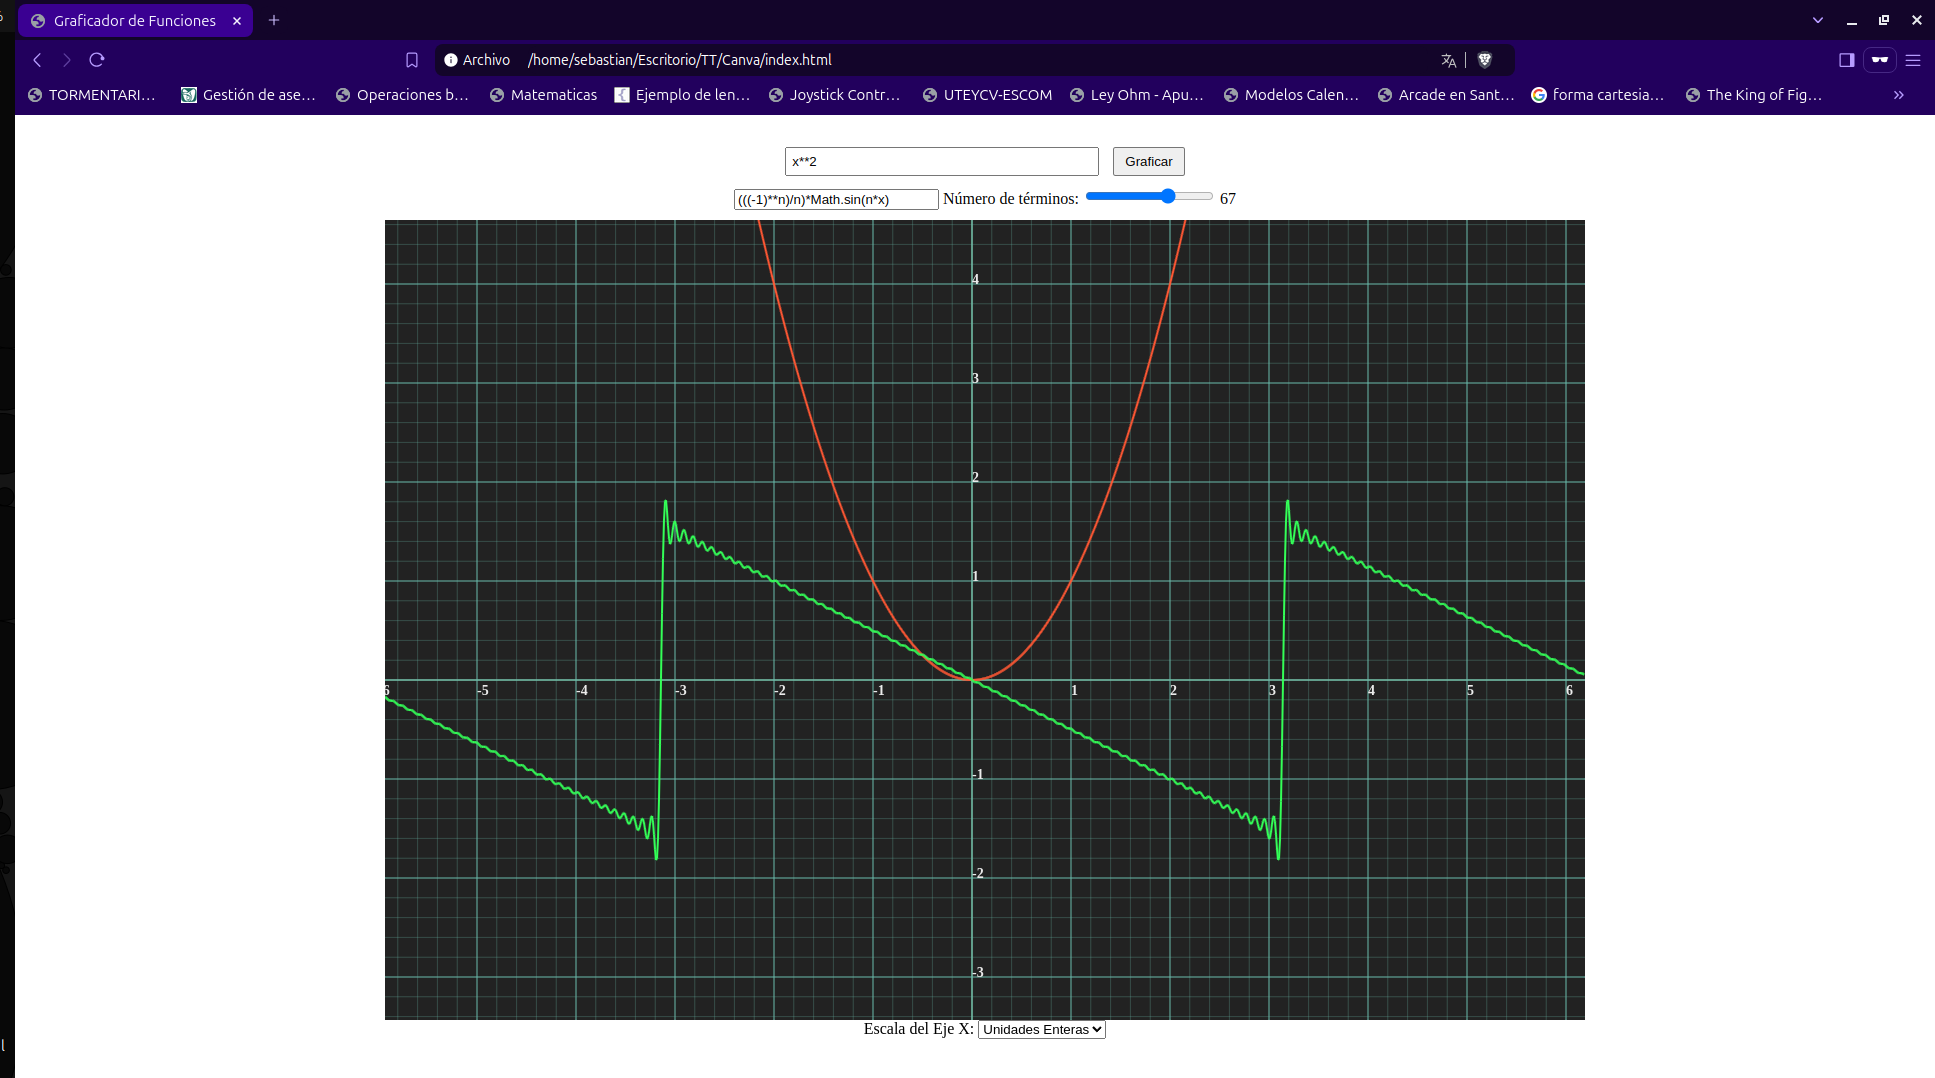
\includegraphics[width=1\textwidth]{img/chapter06/prueba_grafica.png}
	\caption[Plano hecho con un elemento canva.]{Plano hecho con un elemento canva. \textit{Fuente: Elaboración propia}}
	\label{fig:prueba_grafica}
\end{figure}

\section{Programas en Maxima para cálculo matemático}
Lo siguiente fue enfocarse en hacer los cálculos de los coeficientes de ls serie trigonométrica y la extensión de su serie para obtener cada termino (\ref{app3:maxima_trig_proto}) \ref{fig:prueba_maxima_trig}.
\begin{figure}[H]
	\centering
	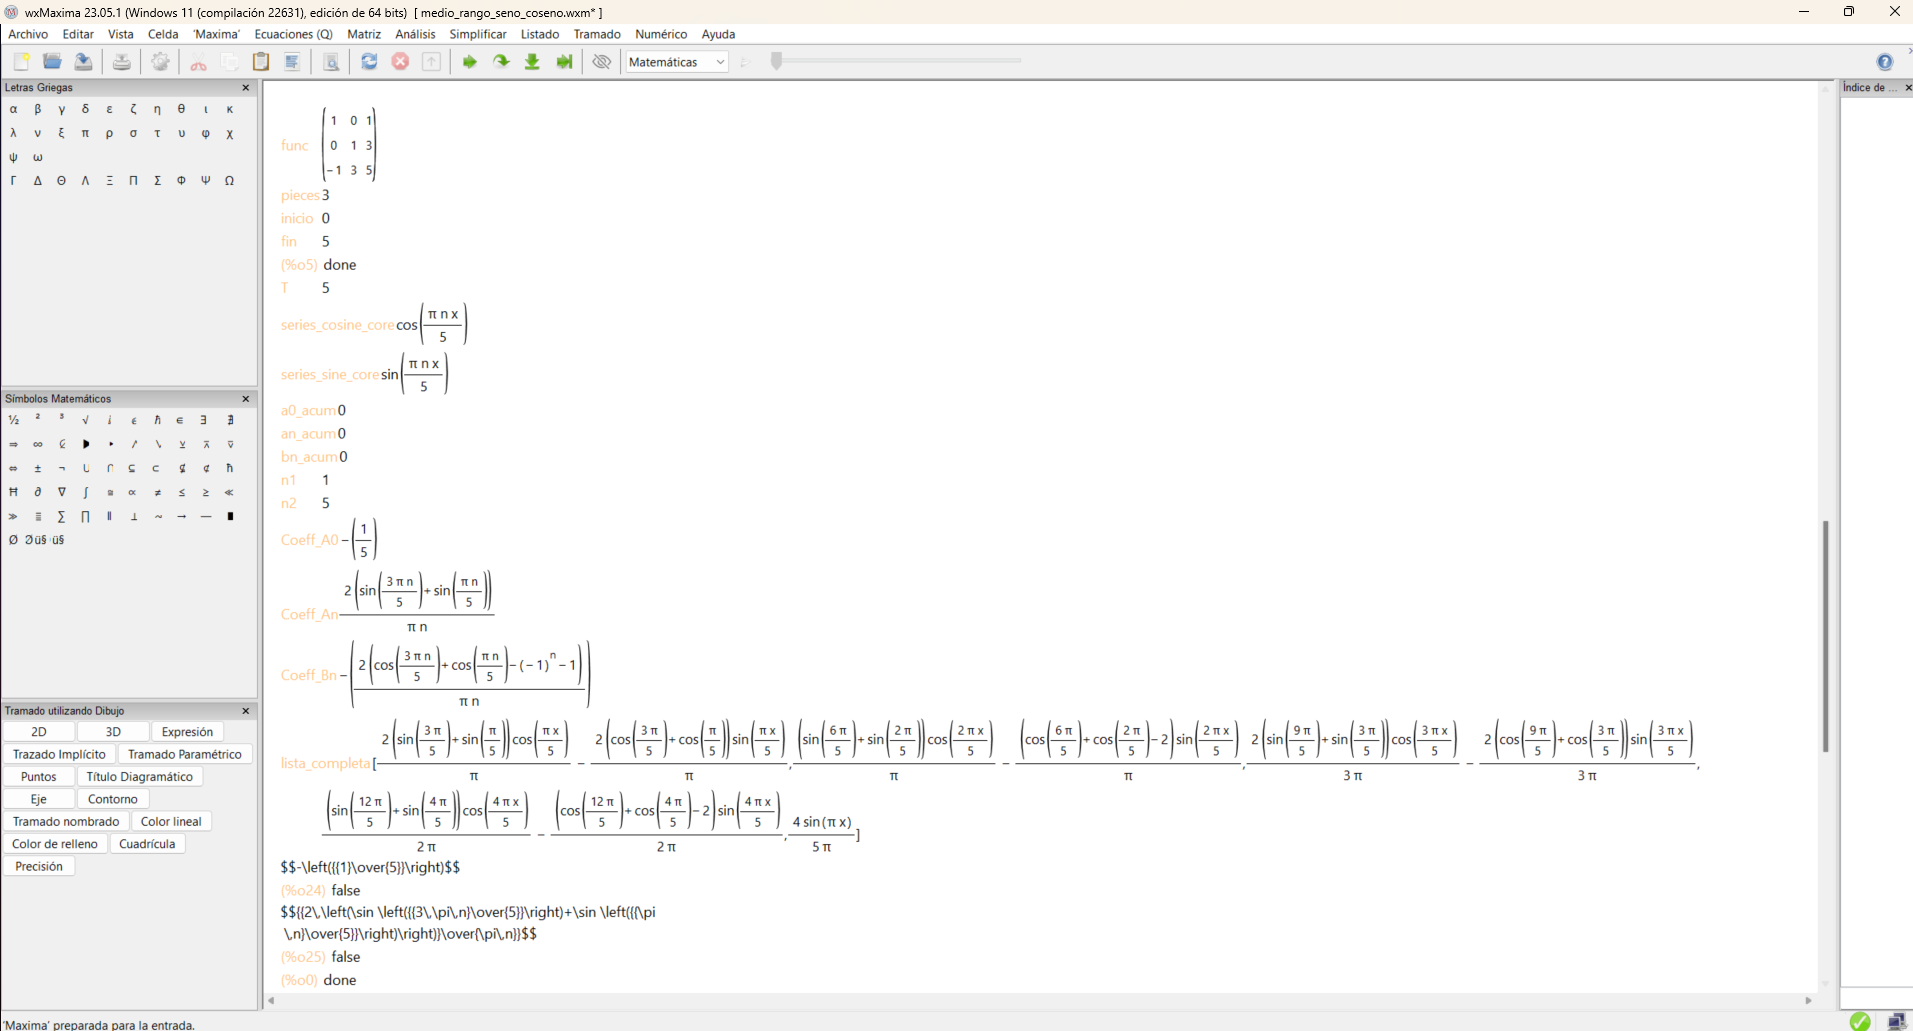
\includegraphics[width=1\textwidth]{img/chapter06/prueba_maxima_trig.png}
	\caption[Código en Maxima para calcular los coeficientes de la serie trigonométrica y \LaTeX.]{Código en Maxima para calcular los coeficientes de la serie trigonométrica y \LaTeX. \textit{Fuente: Elaboración propia}}
	\label{fig:prueba_maxima_trig}
\end{figure}
Sin embargo, la preocupación se tornaba en la serie compleja, ya que al tener números imaginarios su graficación se tronaba complicada, la buena noticia es que Maxima podía separar las partes real e imaginaria de la serie y así, anular la pare imaginaria dejándonos unicamente con su equivalente real, que si podemos graficar(\ref{app3:maxima_complex_proto}) \ref{fig:prueba_maxima_complex}:
\begin{figure}[H]
	\centering
	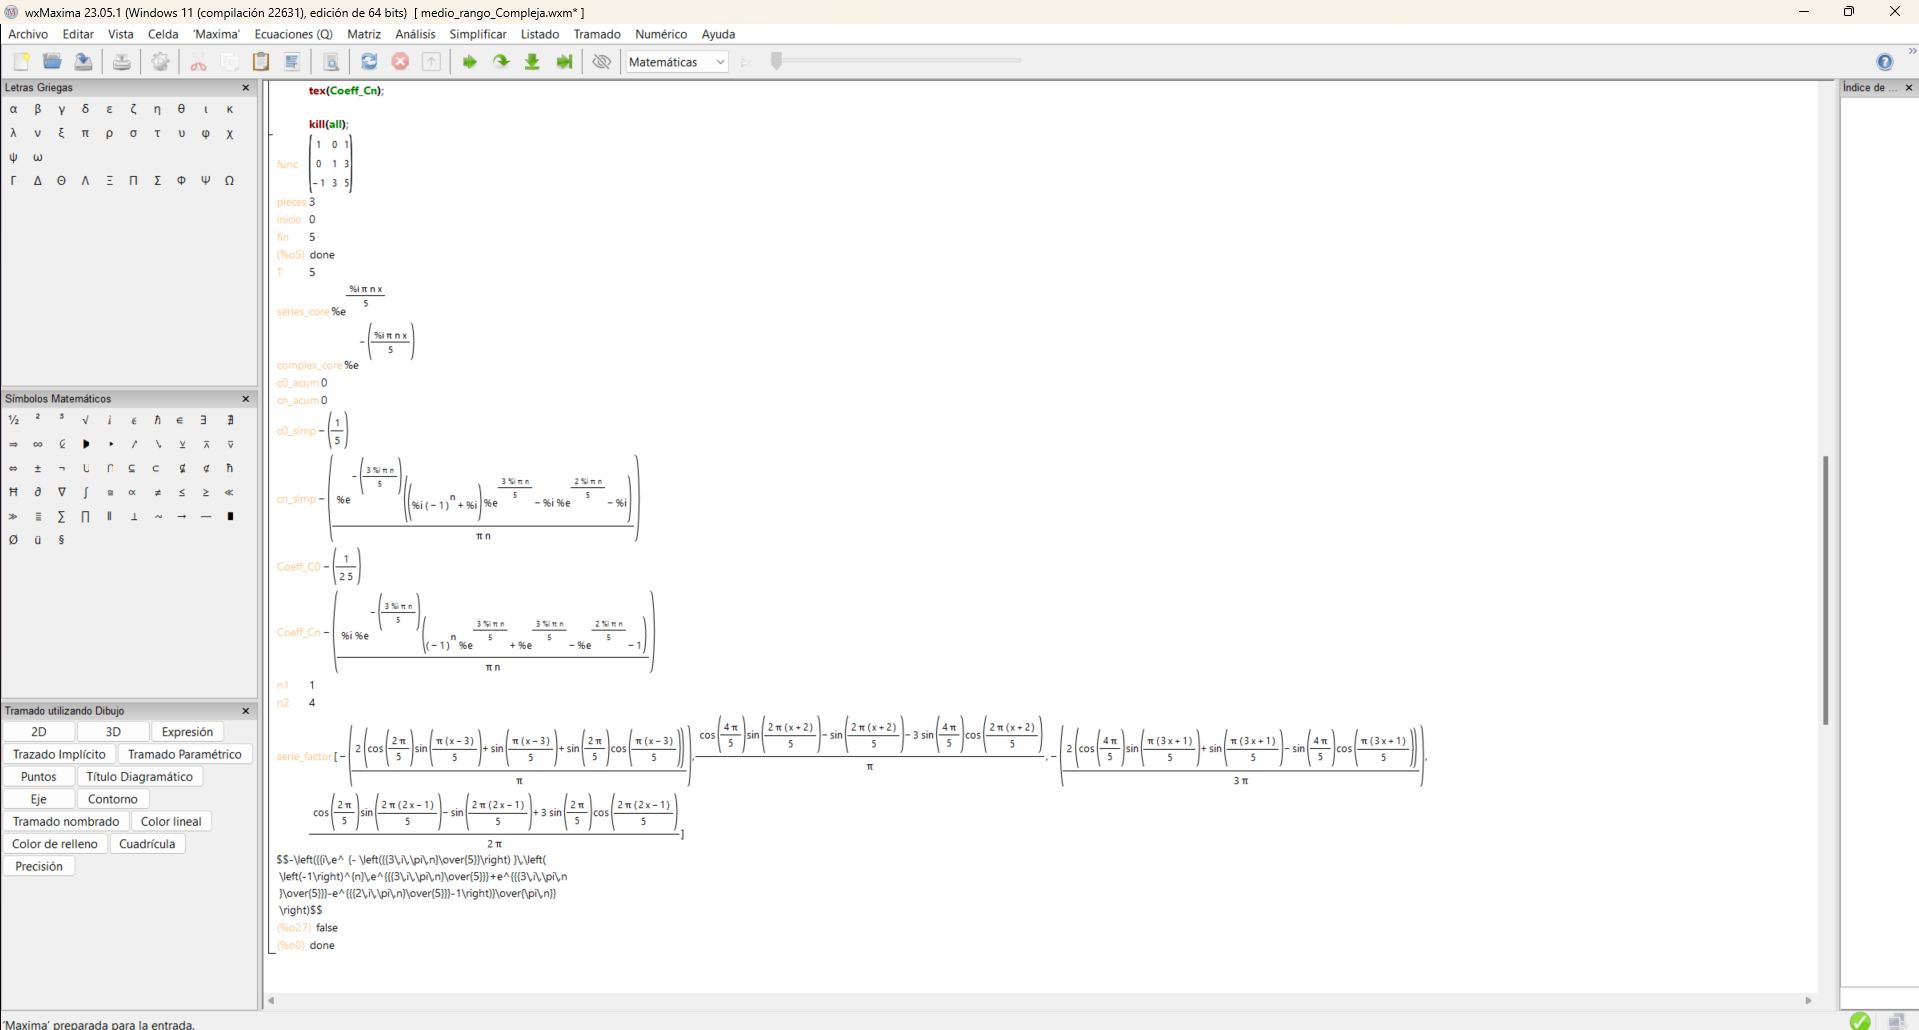
\includegraphics[width=1\textwidth]{img/chapter06/prueba_maxima_complex.png}
	\caption[Código en Maxima para calcular los coeficientes de la serie compleja y \LaTeX.]{Código en Maxima para calcular los coeficientes de la serie compleja y \LaTeX. \textit{Fuente: Elaboración propia}}
	\label{fig:prueba_maxima_complex}
\end{figure}

\section{Creación de una API en Node.js para cálculo}
Una vez comprobamos que Maxima es una gran opción para hacer los cálculos, la siguiente parte fue implementar esta tencología en un lenguaje de servidor para poder llamarlo desde otros proyectos, es decir, crear una API que ejecute a Maxima, para esto se usó NodeJS (\ref{app3:API_nodejs}), ya que al ser un entrono de ejecución en Javascript resultaba ideal por la curva de aprendizaje no tan alta.

\subsection{Pruebas de la API con Postman}
Una vez se tenía la API desarrollada, era turno de probarla, para esto, se usó Postman, para enviar peticiones a la API para solicitar el calculo de los coeficientes de la serie trigonométrica \ref{fig:postman_trig} y exponencial \ref{fig:postman_complex}.
\begin{figure}[H]
	\centering
	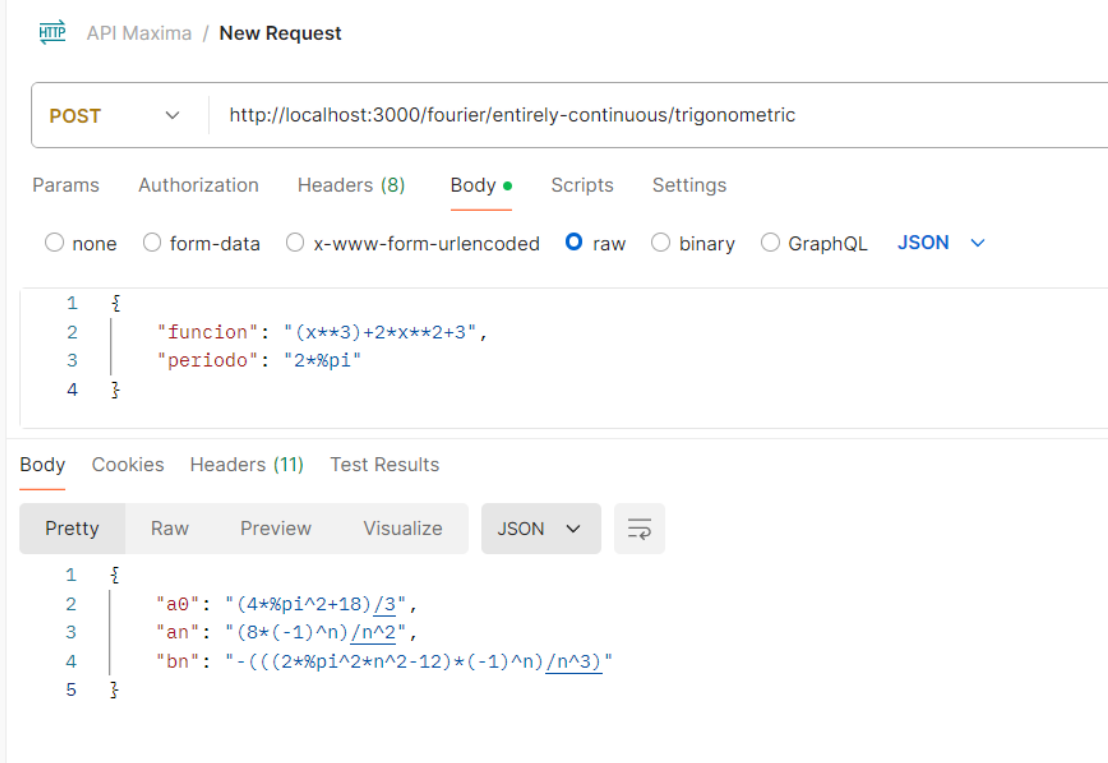
\includegraphics[width=1\textwidth]{img/chapter06/postman_trig.png}
	\caption[Prueba de la API en el endpoint para calcular los coeficientes de la serie trigonométrica.]{Prueba de la API en el endpoint para calcular los coeficientes de la serie trigonométrica. \textit{Fuente: Elaboración propia}}
	\label{fig:postman_trig}
\end{figure}

\begin{figure}[H]
	\centering
	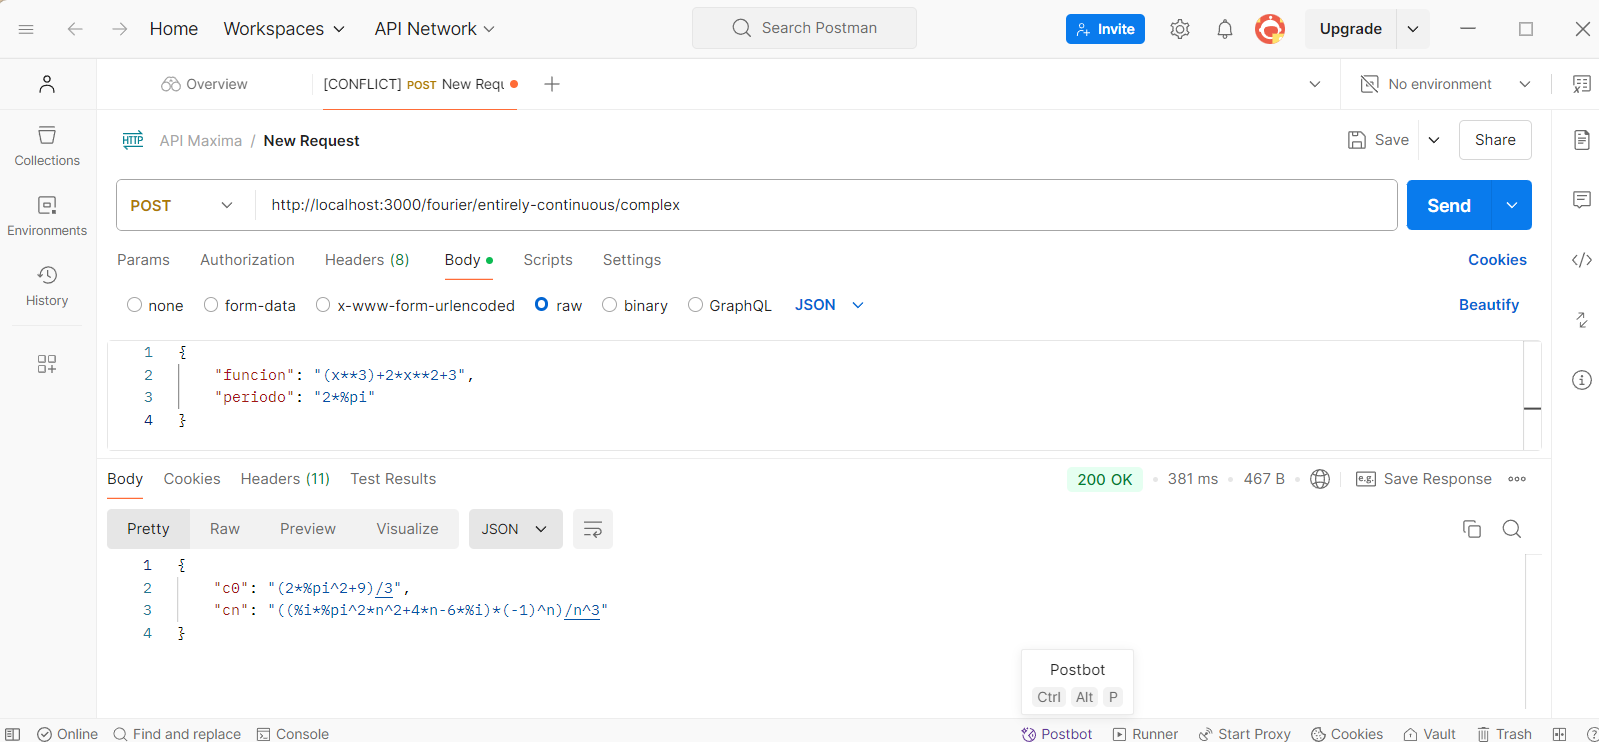
\includegraphics[width=1\textwidth]{img/chapter06/postman_complex.png}
	\caption[Prueba de la API en el endpoint para calcular los coeficientes de la serie compleja.]{Prueba de la API en el endpoint para calcular los coeficientes de la serie compleja. \textit{Fuente: Elaboración propia}}
	\label{fig:postman_complex}
\end{figure}


\section{Pruebas de entradas matemáticas en formato \LaTeX con MathQuill}
Ya teniendo como calcular y graficar, tocó el turno de comenzar con los prototipos de interfaces de usuario, para esto, se propuso MathQuill (\ref{fig:prueba_mathquill})para capturar los datos, al usar \TeX permite una visualización mas agradable de los datos.

\begin{figure}[H]
	\centering
	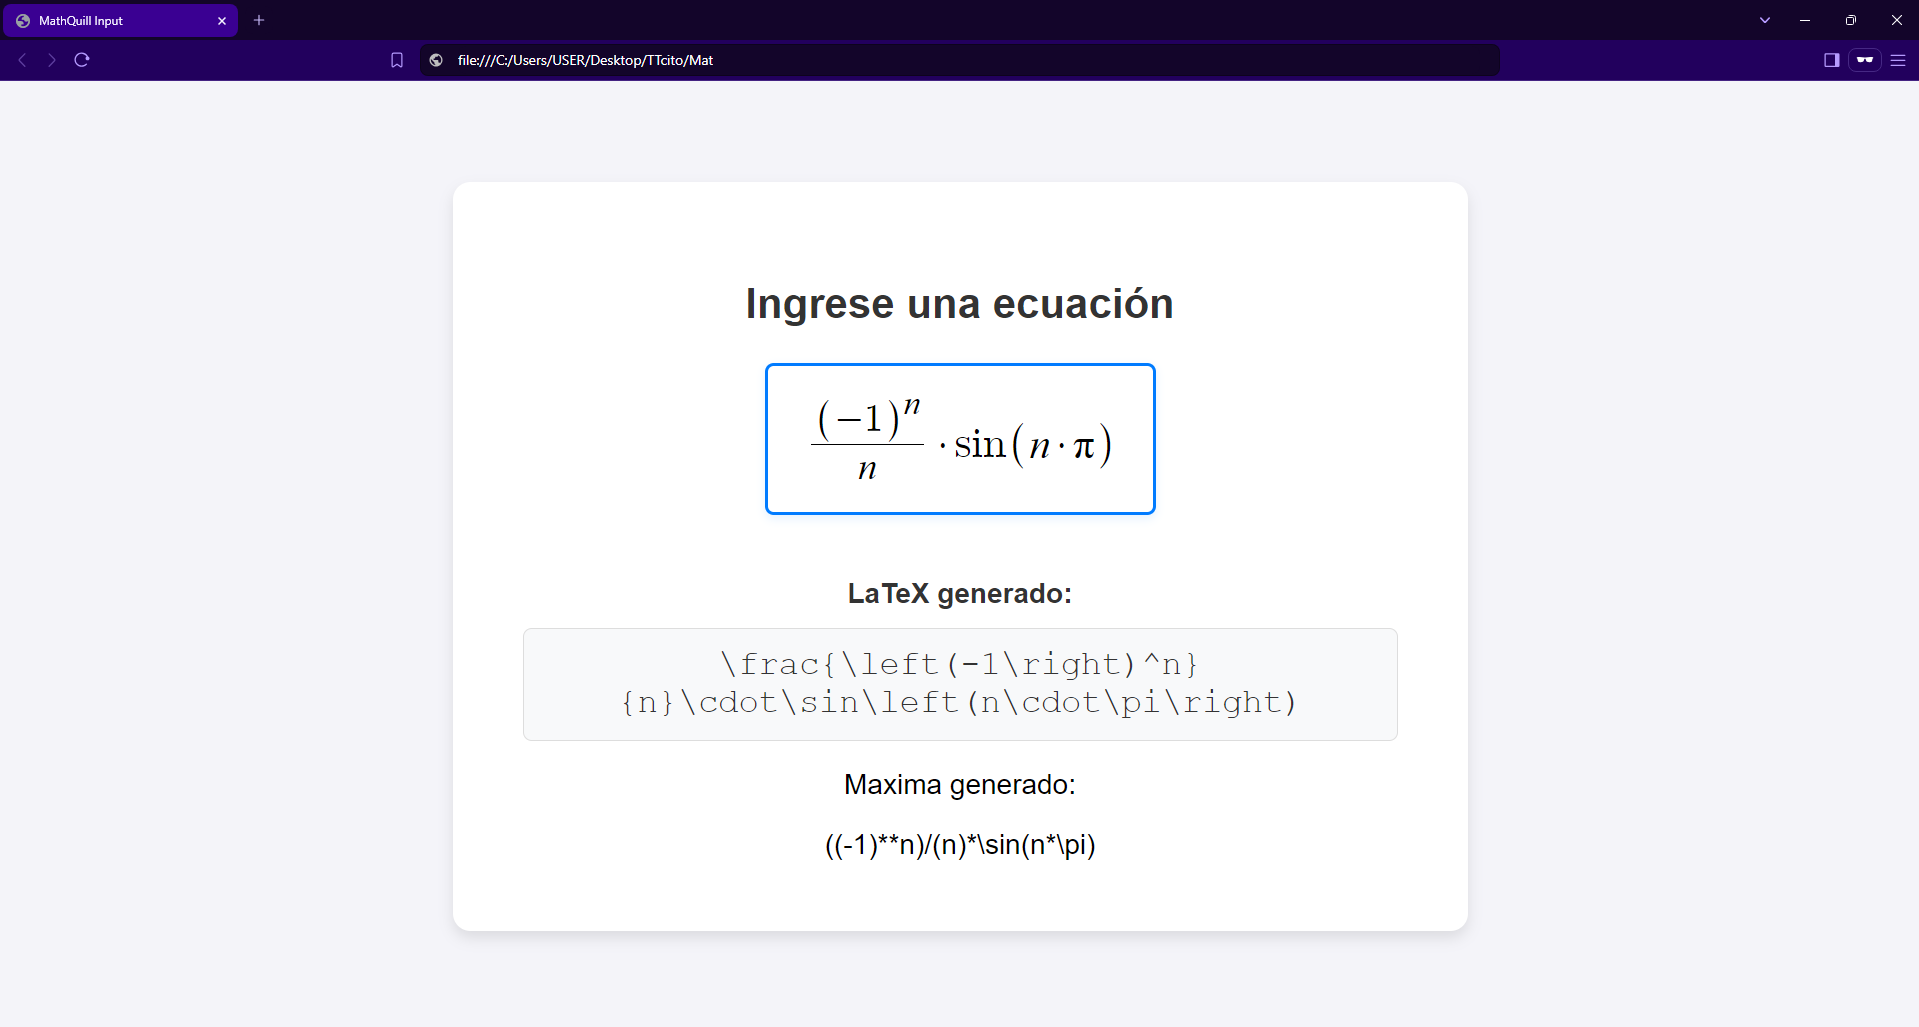
\includegraphics[width=1\textwidth]{img/chapter06/prueba_mathquill.png}
	\caption[Prueba de la biblioteca de MathQuill para el ingreso de funciones.]{Prueba de la biblioteca de MathQuill para el ingreso de funciones. \textit{Fuente: Elaboración propia}}
	\label{fig:prueba_mathquill}
\end{figure}


\section{Creación de un teclado usando MathJax}
Al tener el campo para que el usuario ingrese los datos de su función, surgió el dilema de que los usuarios no tienen porque saber \TeX, así que, usando la biblioteca de MathJax (\ref{app3:mathquill_mathjax_keyboard}), que nos permite a nosotros como desarrolladores, escribir texto en \TeX en nuestro sitio web, con esto en las manos, se diseñó un teclado imitando al de una calculadora, para que el usuario pueda ingresar las funciones válidas y más comunes para las series de Fourier a solo un botón de distancia \ref{fig:prueba_mathquill_mathjax}.

\begin{figure}[H]
	\centering
	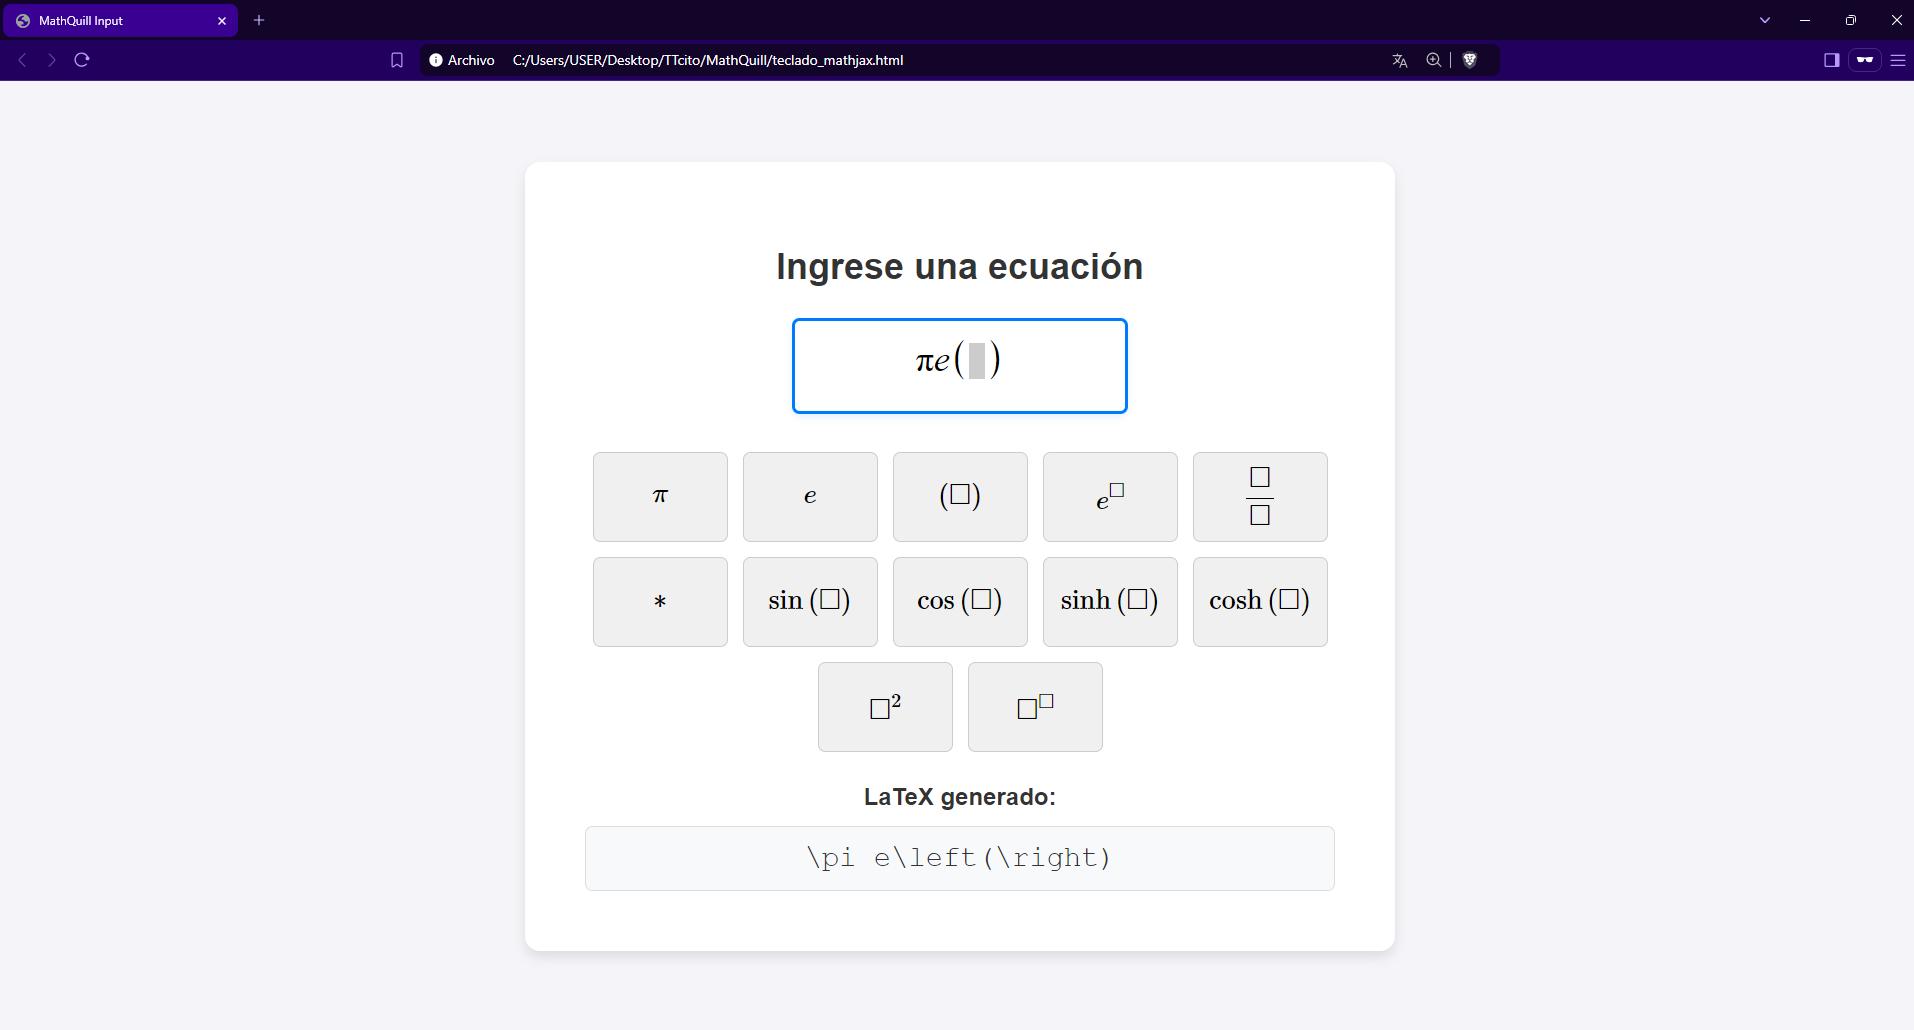
\includegraphics[width=1\textwidth]{img/chapter06/prueba_mathquill_mathjax.png}
	\caption[Prueba de la biblioteca de MathQuill y un teclado hecho en MathJax para el ingreso de funciones.]{Prueba de la biblioteca de MathQuill y un teclado hecho en MathJax para el ingreso de funciones. \textit{Fuente: Elaboración propia}}
	\label{fig:prueba_mathquill_mathjax}
\end{figure}

\section{Prototipo de interfaz de ingreso de funciones}
Ya con lo necesario para una interfaz de ingreso de datos, se comenzó con el diseño inicial de nuestra interfaz para que los usuarios puedan ingresar funciones matemáticas, configurar parámetros y enviar datos para poder calcular una serie de Fourier.

\begin{figure}[H]
	\centering
	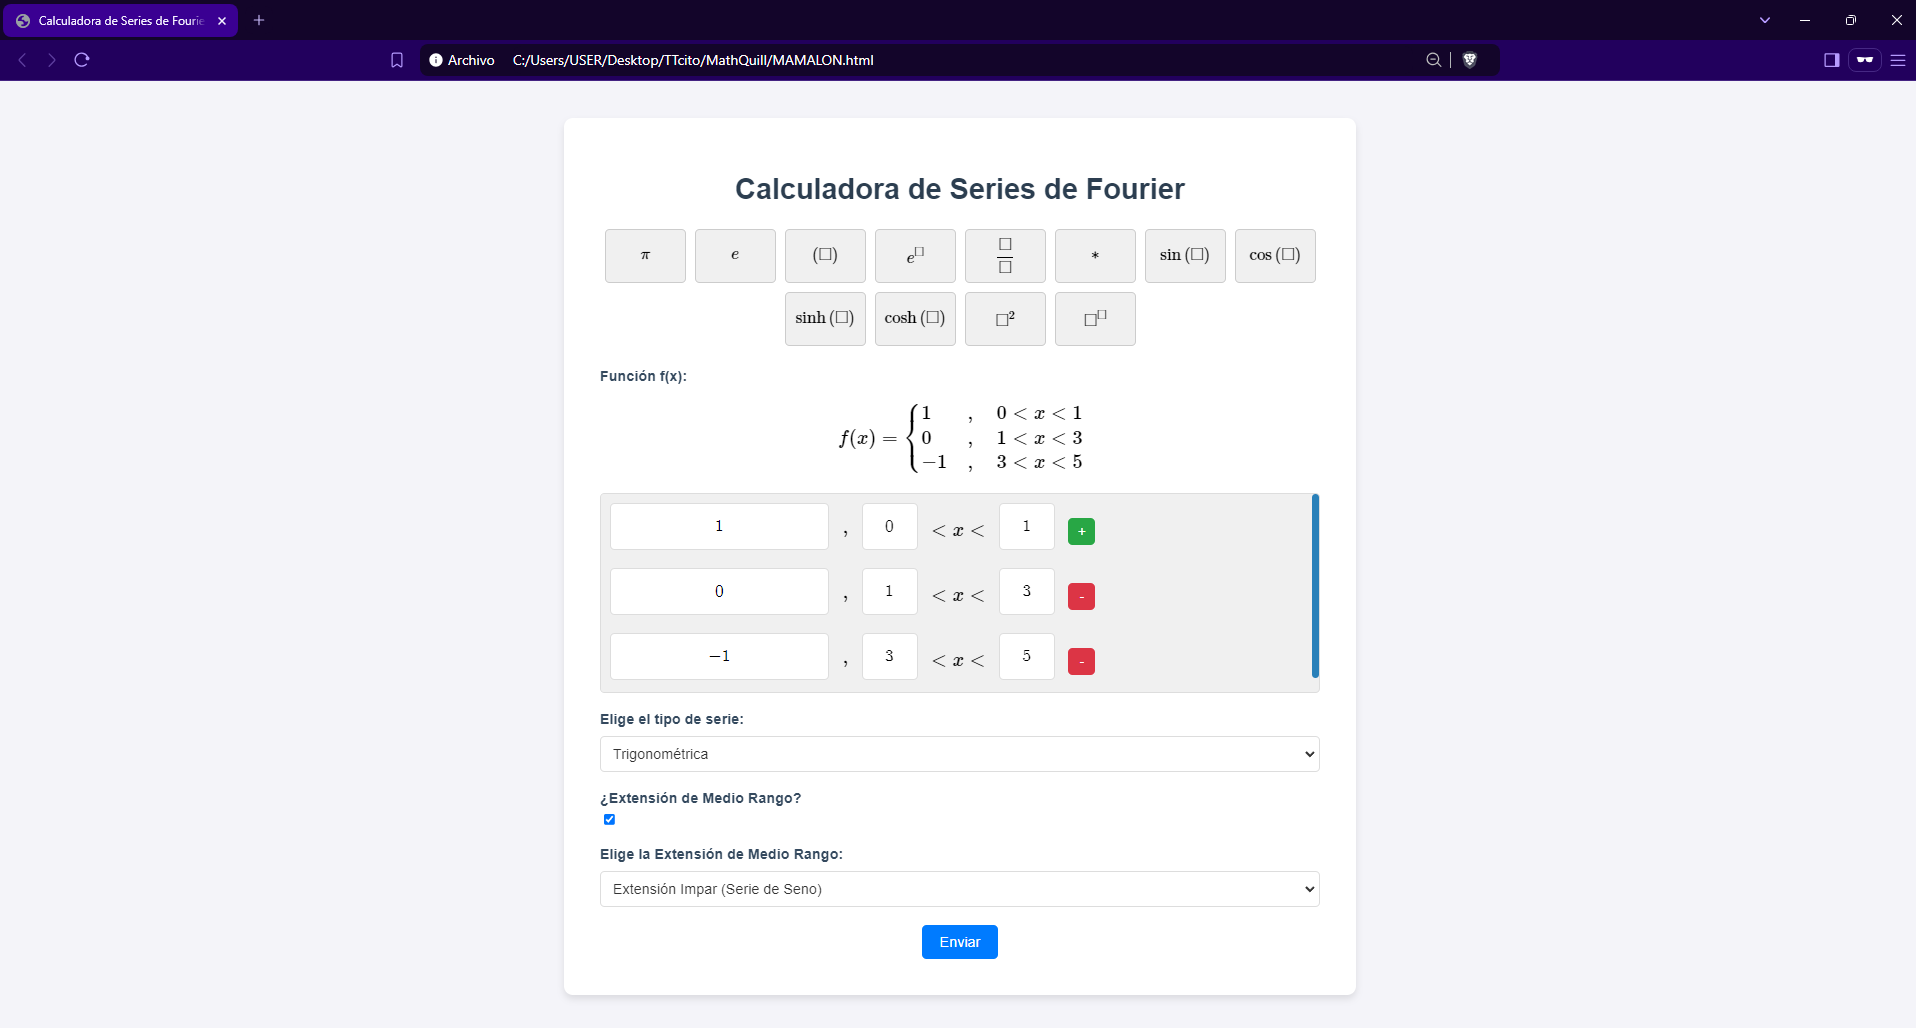
\includegraphics[width=1\textwidth]{img/chapter06/prueba_UI.png}
	\caption[Prototipo de la interfaz de ingreso de funciones.]{Prototipo de la interfaz de ingreso de funciones. \textit{Fuente: Elaboración propia}}
	\label{fig:prueba_UI}
\end{figure}

\section{Pruebas de parseo con tex2max}
Ya teniendo como ingresar los valores, se cayó en cuenta de que lo que envían estos campos son valores en \TeX, y nuestra API funciona con Maxima, aquí es donde se hicieron pruebas con una biblioteca independiente para poder hacer este parseo (\ref{app3:node_js_tex2max}), para comprobar que de verdad este componente funcionaba y sería de utilidad para este proyecto 	\ref{fig:tex2max_node}.
\begin{figure}[H]
	\centering
	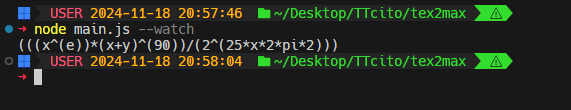
\includegraphics[width=1\textwidth]{img/chapter06/tex2max_node.png}
	\caption[Prueba de la biblioteca de tex2max sobre NodeJS.]{Prueba de la biblioteca de tex2max sobre NodeJS. \textit{Fuente: Elaboración propia}}
	\label{fig:tex2max_node}
\end{figure}

\section{Migración del Canvas a Angular}
Ya teniendo todos los módulos contemplados para el funcionamiento de la aplicación, se procedió a migrar el primero de estos módulos en ser desarrollado, el lienzo al framework de Angular, esto debido a su arquitectura robusta basada en componentes, lo que facilita la reutilización de código y el mantenimiento del proyecto acelerando el proceso de desarrollo. Angular trabaja con un Typescript, un super conjunto de Javascript, por lo que su migración no se tornó complicada \ref{fig:prueba_canva_angular}.

\begin{figure}[H]
	\centering
	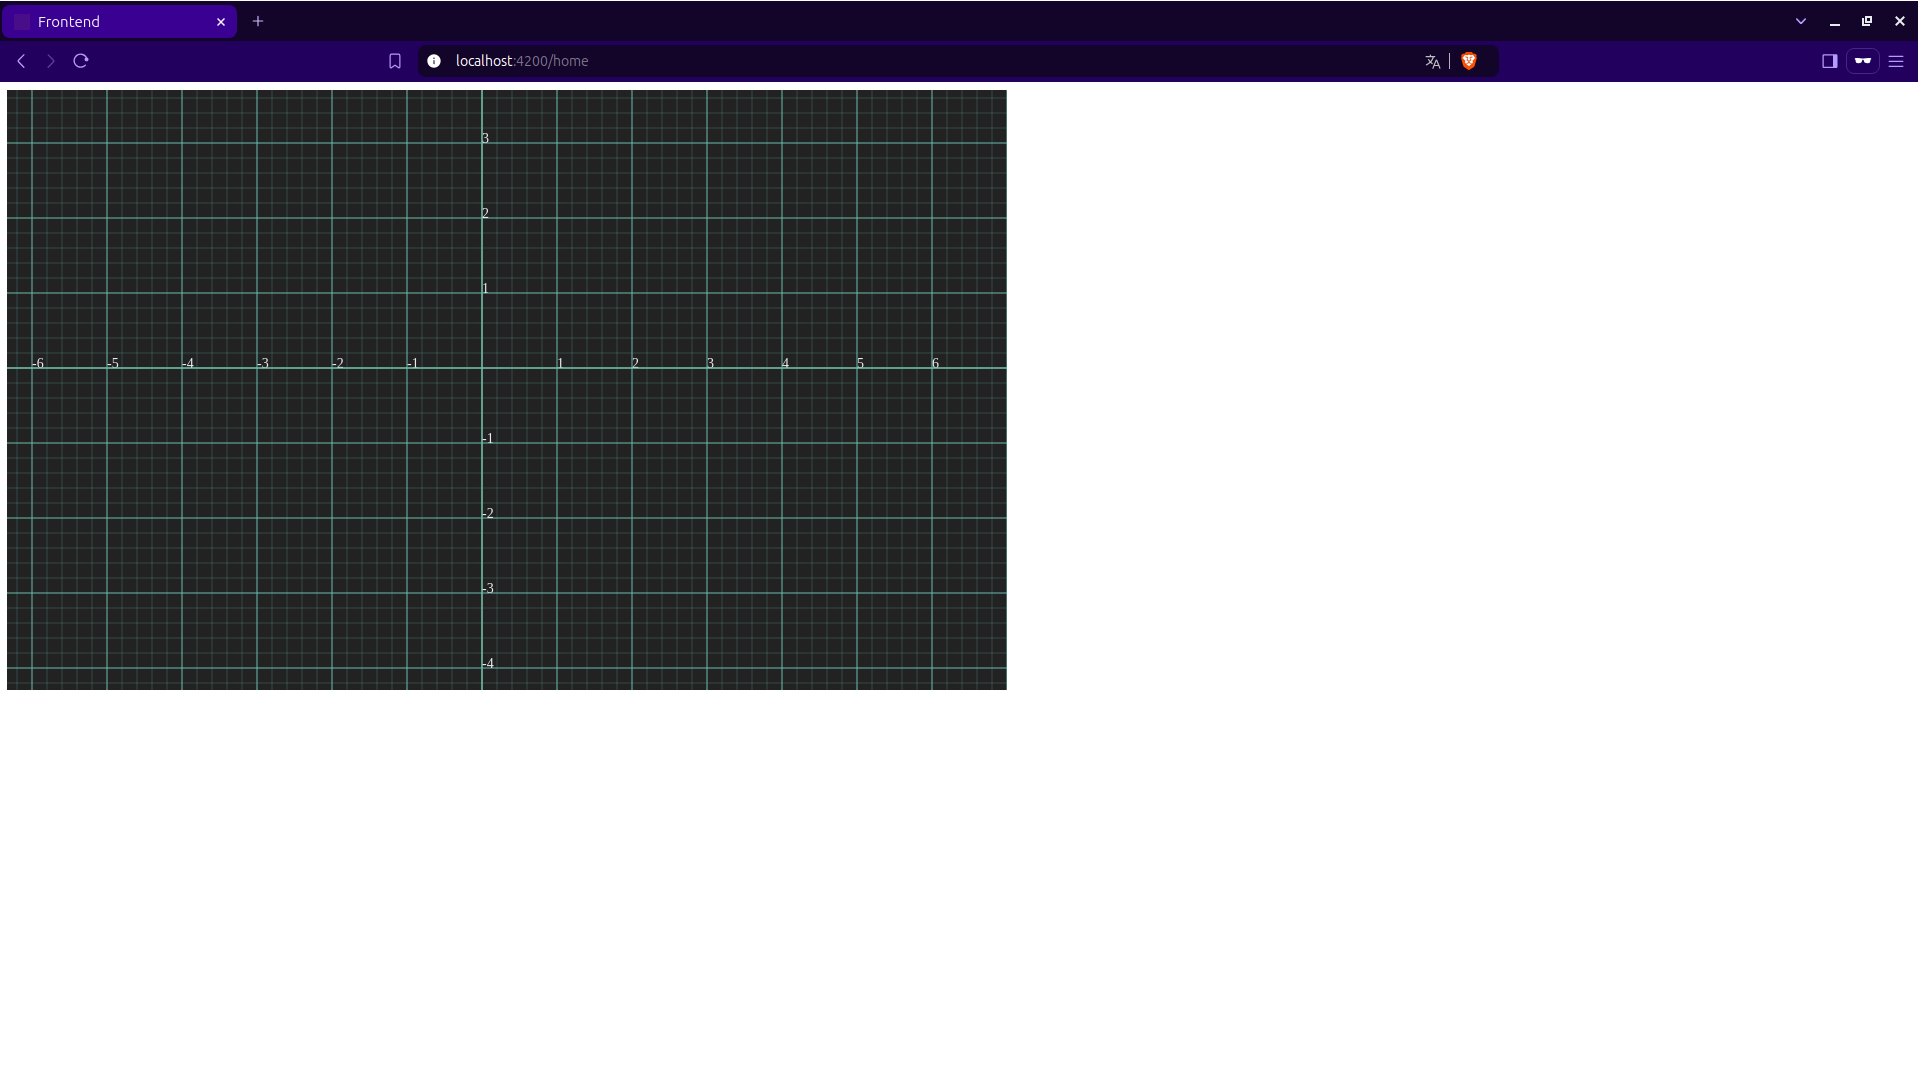
\includegraphics[width=1\textwidth]{img/chapter06/prueba_canva_angular.png}
	\caption[Plano hecho en canva sobre Angular.]{Plano hecho en canva sobre Angular. \textit{Fuente: Elaboración propia}}
	\label{fig:prueba_canva_angular}
\end{figure}

\section{Pruebas de tex2max en Angular}
La última prueba fue el probar una librería de terceros en el framework de Angular, ya que podrían darse incompatibilidades y si, al principio no se reconocía la biblioteca, la solución fue crear un archivo \texttt{.d.ts}, que es una declaración de TypeScript que proporciona información de tipos para bibliotecas JavaScript. Esto permite que permiten que TypeScript entienda las estructuras, funciones y objetos de una biblioteca externa, facilitando así su integración y uso dentro de una aplicación Angular (\ref{fig:tex2max_angular}).
\begin{figure}[H]
	\centering
	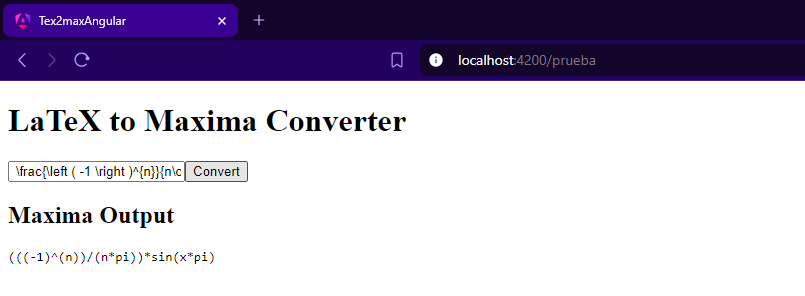
\includegraphics[width=1\textwidth]{img/chapter06/tex2max_angular.png}
	\caption[Prueba de la biblioteca de tex2max en Angular.]{Prueba de la biblioteca de tex2max en Angular. \textit{Fuente: Elaboración propia}}
	\label{fig:tex2max_angular}
\end{figure}